\chapter{Разработка файловых конвертеров в виде приложения <<primiview>>}
\label{cha:entwickl}

Программное обеспечение решено назвать \textbf{<<primiview>>}, где \textbf{<<primi>>} --- сокращение от англ. \textit{primitive} (\textit{примитив}), \textbf{view} --- в переводе с англ. \textit{обзор}.

В данном разделе описаны экономические аспекты проекта по созданию ПО <<primiview>> для обработки геометрической информации 2D-объектов специального типа.

\section{Выбор языка программирования}
Для написания программы выбран язык программирования Python версии 3.11. Выбор языка программирования обоснован несколькими факторами.

\paragraph{Библиотеки.} Для создания описанного ПП необходимо привлечение различных библиотек. Кроме стандартной библиотеки, с Python можно использовать множество прикладных библиотек, несколько из которых будут описаны в следующих частях работы. Специфичные библиотеки, позволяющие <<читать>> DXF-файл и обрабатывать содержимое внутри него, написаны не для каждого ЯП. Библиотека <<eazy dxf>> для Python позволяет быстро и удобно выполнять данные операции.

\paragraph{Кроссплатформенность.} Большинство программ, написанных на Python, выполняются корректно на всех основных платформах. Перенос программы между операционными системами реализуется простым копированием кода. Кроме того, в процессе разработки ПО, для реализации пользовательского интерфейса используется набор расширений Qt, который тоже работает на таких платформах, как Linux и другие UNIX-подобные ОС, macOS и Windows.

\paragraph{Скорость и удобство разработки.} Удобочитаемсть, ясность и высокое качество этого языка позволяют повысить производительность разработчика во много раз, сравнивая, например, с компилирующими или строго типизированными языками, такими как C, C++ и Java. Объём программного кода на языке Python обычно составляет треть или даже пятую часть эквивалентного программного кода на языке C++ или Java. Кроме того, при запуске программы, написанной на ЯП Python минуются длинные этапы компиляции и связывания, необходимые в некоторых других ЯП, что, также, увеличивает производительность труда программиста \cite{ascher2004learning}.

В ходе сравнительного анализа языков программирования для использования особое внимание уделялось чтению DXF. В тоткрытом доступе были найдены библиотеки для Python (\textit{ezdxf}), C\#(\textit{netDxf}), для C++ и других языков были найдены исходные коды, позволяющие обрабатывать DXF-файлы.

В итоге, учитывая вышеприведённые аспекты-преимущества языка Python, а также относительно большой опыт работы по написанию ПО на этом языке, в сравнении с другими, учитывая крайне высокую степень разработки библиотеки \textit{ezdxf} было принято решение использовать язык Python и библиотеку \textit{ezdxf} для разработки ПО.


\section{Принцип работы приложения <<primiview>>}

Для создания программного обеспечения необходимо сначала разработать концепцию функционирования программы, опираясь на её назначение, на основные её функции. Когда определены модули, блоки и функциональные части ПО, можно приступать к разработке его на выбранном ЯП.

Основываясь на цели, поставленной во введении, разрабатываемая утилита должна принимать на входе DXF-файл, то есть открывать его и обрабатывать его содержимое. Для проверки правильности обработанных данные, то есть, для верификации содержимого DXF-файла, программа должна визуализировать для пользователя обработанное. После верификации обработанных данных и, соответственно, подтверждения соответствия их исходным, пользователю должна предоставляться возможность конвертировать эти данные в какой-либо из предлагаемых форматов. За это отвечает модуль экспорта, который, в свою очередь, подразделяется на четыре модуля, отвечающие за преобразование данных в различные форматы. Среди них следующие:

\begin{enumerate}
	\item Модуль экспорта в TXT-файл, где данные будут представлены в такой же форме, как и в оригинальном DXF-файле, за исключением того, что содержаться в нём будут только поддерживаемые сущности (LINE, POLYLINE, ARC, CIRCLE).
	\item Модуль экспорта в TXT-файл, в котором поддерживаемые сущности будут представлены сочетанием двух строк, первая из которых --- начальная точка примитива, вторая --- конечная. Вторая строка содержит в себе радиус скругления примитива, переходящего из первой точки во вторую.
	\item Модуль экспорта в формат SVG, который, при открытии, векторно отображает информацию в нём.
	\item Модуль экспорта JSON-формат. В данном формате, по подобию формату TXT (x, y, r), содержаться точки, олицетворяющие начало и конец того или иного примитива. В данном случае информация в файле тэгированная, что означает, что в дальнейшем несложно будет получить желаемые куски данных из потенциально объёмного JSON-файла путём обращения по желаемому тэгу.
\end{enumerate}


Схему, отображающую основное содержание разрабатываемого ПО, можно наблюдать на рисунке \ref{fig:organisationsdiagramm}.

\begin{figure}[H]
	\centering
	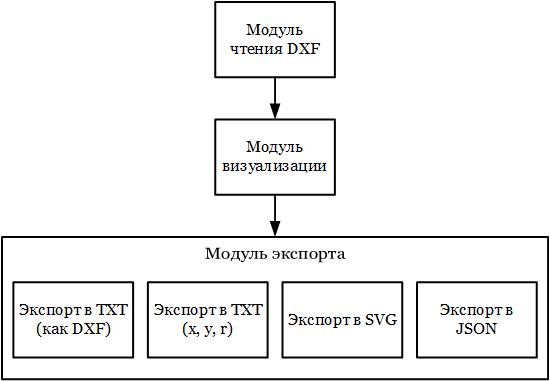
\includegraphics[width=0.8\textwidth]{figures/organisationsdiagramm.png}
	\captionof{figure}{Принципиальная структура ПО <<Primiview>>}
	\label{fig:organisationsdiagramm}
\end{figure}

\section{Внутрепрограммная репрезентация информации о геометрических примитивах}
Учитывая то, что проблема с работой по чтению входных DXF-файлов решена с помощью библиотеки \textit{ezdxf}, задача разработки ПО фактически свелась к внутренней респезентации необходимой геометрической информации внутри программы для дальнейшей работы с ней.

Есть несколько вариантов хранения геометрических данных в программе на ЯП Python: списки, словари и классы.

В списках обычно хранятся объекты одного типа (например, только координаты в виде чисел). Это не удовлетворяет потребности обмена данными, так как нужная геометрическая информация из DXF содержит в себе и строковые, и булевы значения, а также другие типы данных.

Словари обеспечивают более простой и понятный доступ к полям, чем списки (то есть не по числовым индексам, а по ключам). Однако словари имеют некоторые ограничения, которые могут оказаться существенными по мере разработки программы.

Во-первых, в словарях не предусмотрено место для централизованного хранения логики обработки записей. Это допустимо в разрабатываемом ПО, так как функции работы с геометрическими примитивами в частях программы имеют одинаковый характер, поэтому не требуется прописывать поведение каждого класса объектов \cite{lutz2001programming}.

Однако недостаток использования словарей для представления записей, заключающийся в том, что со временем их становится трудно расширять, является решающим при выборе типа данных для хранения информации о геометрических примитивов. Так как ПО <<primiview>> требуется постоянно модифицировать для работы с новыми файловыми форматами, то основные изменения исходят из взятия из исходных DXF-файлов дополнительной информации для её последующей обработки. Поэтому сложность дополнения словарей новой информацией недопустима при разработке данного ПО.

Кроме прочих преимуществ хранения данных с помощью классовых свойств, ценна возможность создания списков внутри классов, которые позволяют объединять одноротную по типу информацию, что упрощает её дальнейшую обработку.

Таким образом, учитывая вышеприведённые аргументы, а также следуя принципам объектно-ориентированного программирования (ООП) в разработке ПО, принято решение хранить каждый примитив в виде объекта класса этих примитивов.

Предусмотрен отдельный класс данных (\textit{DxfData}), работающий с примитивами, извлечёнными из DXF. Он содержит в себе списки объектов соответствующих классов (линия, дуга, др.), а также методы (функции внутри класса) по работе с ними.

Схема, отображающая структуру хранения данных из DXF-файлов внутри программы приведена на рисунке \ref{fig:classes}.

\begin{figure}[H]
	\centering
	\includegraphics[width=1.0\textwidth]{figures/classes.png}
	\captionof{figure}{Структура хранения данных в ПО <<primiview>>}
	\label{fig:classes}
\end{figure}


\section{Разработка алгоритмов} \label{sec:algs}
Алгоритм \ref{alg:readdxf} показывает схему работы процесса извлечения поддерживаемых ПО Primiview примитивов из выбранного DXF-файла.

На первой итерации осуществляется разбиение блоков, в которых могут быть <<спрятаны>> остальные сущности. В случае, если пропустить данный этап, то объекты, находящиеся внутри блоков не будут видны библиотекой \textit{ezdxf}, которая используется для чтения DXF-файлов.

После <<разрушения>> всех блоков примитивы становятся <<видимыми>>. Далее запускается цикл, итерирующий объекты пространства объектов модели (\textit{modelspace}). В случае совпадения объекта с одной из поддерживаемых сущностей, она сохраняется в список соответствующих объектов в оперативной памяти программы. Списком далее будет называться изменяемый упорядоченный тип данных, представляющих собой последовательность элементов, разделённых между собой запятой и заключённых в квадратные скобки. Данный тип данных используется в ЯП Python.

Примем ряд условных обозначений:

$\rightsquigarrow$ --- запись в файл;
$\dashrightarrow$ --- запись объекта в множество.


\begin{algorithm}[H]
	\SetAlgoLined
	\KwData{путь к DXF-файлу}
	\KwResult{массивы примитивов и информации о них в оперативной памяти программы}
	инициализация;
	
	\ForEach{объекта типа Вставка (INSERT) $\in msp$}{разбиение сущности}
	
	\ForEach{объекта $\in msp$}{
		\If{объект явл. линией}{объект. $\dashrightarrow$ множ. линий}
		\ElseIf{объект явл. дугой}{объект $\dashrightarrow$ множ. дуг}
		\ElseIf{объект явл. окружностью}{объект $\dashrightarrow$ множ. окружностей}
		\ElseIf{объект явл. полилинией}{объект $\dashrightarrow$ множ. полилиний}
	}
	
	\caption[Сохранение поддерживаемых примитивов; из DXF в оперативную память программы]
	{\tabular[t]{@{}l@{}}Сохранение поддерживаемых примитивов \\ из DXF в оперативную память программы\endtabular}
	\label{alg:readdxf}
\end{algorithm}

\paragraph{Алгоритм записи примитивов в TXT (как DXF).} Принцип данного алгоритма (см. алгоритм \ref{alg:dxfintotxt}) основан на открытии созданного TXT-файла, а после --- перебора прочитанных из DXF примитивов и записи из каждого из них необходимой информации в открытый для редактирования TXT-файл.

Записи в текстовом файле должны выглядеть следующим образом (см. листинг \ref{list:txtdxfsicht}):
%\begin{verbatim}
%	LINE(#01)
%	0.1 0.1
%	0.1 0.1
%\end{verbatim}

\begin{lstlisting}[caption={Пример содержания TXT-файла (как DXF)},label=list:txtdxfsicht]
	LINE(#01)
	0.1 0.1
	0.1 0.1
\end{lstlisting}

\begin{algorithm}[H]
	\SetAlgoLined
	\KwData{данные из DXF, путь к имя.txt}
	\KwResult{имя.txt (как DXF)}
	инициализация;
	\ForEach{LINE}{атрибут сущности, $x_0, y_0$, $x_1, y_1 \rightsquigarrow$имя.txt}
	\ForEach{ARC}{атрибут сущности, $x_0, y_0$, $x_1, y_1$, $r\rightsquigarrow$имя.txt}
	\ForEach{CIRCLE}{атрибут сущности, $x_c, y_c$, $r\rightsquigarrow$имя.txt}
	\ForEach{LWPOLYLINE}{атрибут сущности;\\
		\ForEach{LWPOLYLINE}{
			\ForEach{координата}{координата$\rightsquigarrow$имя.txt}
		}}
	\caption{Запись примитивов в TXT (DXF-type)}
	\label{alg:dxfintotxt}
\end{algorithm}

В алгоритме \ref{alg:dxfintotxt} $x_0, y_0$ --- координаты начала примитива; $x_1, y_1$ --- координаты конца примитива; $x_c, y_c$ --- координаты центра окружности; $r$ --- радиус дуги или окружности.

\paragraph{Алгоритм записи примитивов в TXT (x,y,r).} Алгоритм \ref{alg:primsintotxt} призван, так же как и в прошлом случае, в открытый только что созданный текстовый файл записать информацию о примитивах, которые были прочитаны из выбранного DXF-файла.

Записи в текстовом файле должны выглядеть следующим образом (см. листинг \ref{list:primsdxfsicht}):
%\begin{verbatim}
%	1.52 1.86 0
%	1.12 2.08 0
%	1.16 2.04 4.0
%	...
%\end{verbatim}

\begin{lstlisting}[caption={Пример содержания TXT-файла (x, y, r)},label=list:primsdxfsicht]
	1.52 1.86 0
	1.12 2.08 0
	1.16 2.04 4.0
\end{lstlisting}

Полилиния может содержать в себе, как отрезки, так и дуги. В объектах LWPOINT сущности LWPOLYLINE степень искривления показывает параметр \textit{bulge}, суть которого подробно описана в разделе \ref{sec:arcs}. Так как желаемый формат вывода информации о примитивах содержит именно радиус примитива, а не параметр искривления, то необходимо удобно получить радиус из \textit{bulge}.

Для этого воспользуемся уже выведенной зависимостью \cite{ukoloff} и применим её в принятых обозначениях (\ref{F:rad}):

\begin{equation}
	R=|bulge+\frac{1}{bulge}|\cdot\frac{|A-Z|}{4},
	\label{F:rad}
\end{equation}

где A --- начальная точка;

Z --- конечная точка.

Примем, что $A(x_0,y_0), B(x_1,y_1)$. Тогда $AZ(x_1-x_0; y_1-y_0)$.
Таким образом, длина вектора через декартовы координаты (\ref{F:veclen}):
\begin{equation}
	|A-Z|=\sqrt{(x_1-x_0)^2+(y_1-y_0)^2}
	\label{F:veclen}
\end{equation}


\begin{algorithm}[H]
	\SetAlgoLined
	\KwData{текущая точка, следующая точка}
	\KwResult{радиус сегмента полилинии}
	инициализация;
	
	\If{$bulge$ (текущей точки) $=0$}{$r=0$}	
	\Else{$r=|bulge+\frac{1}{bulge}|\cdot\frac{\sqrt{(x_{nexP}-x_{prevP})^2+(y_{nexP}-y_{prevP})^2}}{4}$}
	
	\caption{Вычисление радиуса сегмента полилинии}
	\label{alg:polyarcrad}
\end{algorithm}

\begin{algorithm}[H]
	\SetAlgoLined	
	\KwData{данные из DXF, путь к имя.txt}
	\KwResult{имя.txt (x,y,r)}	
	\ForEach{LINE}{$x_0 \quad y_0 \quad 0\rightsquigarrow$ имя.txt; \quad $x_1 \quad y_1 \quad 0 \rightsquigarrow$ имя.txt}
	
	\ForEach{ARC}{$x_0 \quad y_0 \quad 0\rightsquigarrow$ имя.txt; \quad $x_1 \quad y_1 \quad r \rightsquigarrow$ имя.txt}
	
	\ForEach{CIRCLE}{$x_c + r \quad y_c \quad 0\rightsquigarrow$ имя.txt\tcc*{первая половина окруж.} $x_c - r \quad y_c \quad r \rightsquigarrow$ имя.txt \\  $x_c - r \quad y_c \quad 0 \rightsquigarrow$ имя.txt\tcc*{вторая половина окруж.} $x_c + r \quad y_c \quad r \rightsquigarrow$ имя.txt} \ForEach{POLYLINE\\ prevPoint=None \tcc*{предыдущая точка}}{
		\ForEach{LWPOINT $\in$ множ. точек полилинии}{
			\If{prevPoint$\neq$None}{r = алгоритм \ref{alg:polyarcrad} (prevPoint, LWPOINT)
				$x(prevP) \quad y(prevP) \quad 0 \rightsquigarrow$ имя.txt\\
				$x(lwpoint) \quad y(lwpoint) \quad r \rightsquigarrow$ имя.txt
			}
			$prevPoint = lwpoint$
		} \newpage
		\If{контур замкнут}{
			r = алгоритм \ref{alg:polyarcrad} (prevPoint, LWPOINT) \\
			$x(lwpoint_\text{посл}) \quad y(lwpoint_\text{посл}) \quad 0 \rightsquigarrow$ имя.txt\\
			$x(lwpoint_\text{перв}) \quad y(lwpoint_\text{перв}) \quad r \rightsquigarrow$ имя.txt
		}
	}
	\caption{Запись примитивов в TXT (x, y, r)}
	\label{alg:primsintotxt}
\end{algorithm}

\paragraph{Алгоритм записи примитивов в SVG.} Формирования файла типа SVG отличается от предыдущих двух, так как этот формат представляет собой язык разметки, а значит, имеет правила синтаксиса, грамматики и т.д. Это расширение языка разметки XML, поэтому в начале, в преамбуле, указывается версия XML, кодировка символов и указание синтаксическому анализатору об игнорировании любых объявлений разметки в определении типа документа.

\begin{lstlisting}[language=XML,caption={Первая строка SVG-файлов},label=list:1stsvgline]
	<?xml version="1.0" encoding="UTF-8" standalone="no"?>
\end{lstlisting}

Следующие две строки должны содержать определение типа документа (заголовок DOCTYPE), однако, данное объявление может оказаться источником ошибок при применении в браузере Mozilla Firefox. Поэтому вместо этого используется атрибут \Code{baseProfile} со значением <<full>> внутри элемента <svg>.

Начиная с четвёртой строки объявляется корневой элемент <svg>:

\begin{lstlisting}[language=XML,caption={Первая строка SVG-файлов},label=list:4thsvgline]
	<svg version="1.1" width="100%" height="100%"
	viewBox="102.1188828597992 -211.7921423734452 50.000000000000014 26.0"
	baseProfile="full"
	xmlns="http://www.w3.org/2000/svg"
	xmlns:xlink="http://www.w3.org/1999/xlink"
	xmlns:ev="http://www.w3.org/2001/xml-events">
\end{lstlisting}

В листинге \ref{list:4thsvgline} присутствует необязательный элемент \Code{viewBox}, который представляет собой параметр с четырьмя значениями, отделяемыми пробелами, определяющими квадратную рамку, в которой будет располагаться графика. Данный атрибут позволяет автоматически масштабировать изображение до размеров указанного контейнера, причём, без потери качества, так как графическая информация храниться и воспроизводится в векторном формате.

Первые два значение --- минимальные координаты $x$ и $y$ рамки, в которой располагается изображение. Третье и четвёртое значения --- соответственно, ширина и высота рамки, в которой находится изображение. Значения указываются в пикселях.

Таким образом, чтобы перенести данные из DXF в SVG, сначала определяются эти четыре значения. Алгоритмы для их определения: алгоритм \ref{alg:allcoords}, алгоритм \ref{alg:extremums} и алгоритм \ref{alg:dimes}.

\begin{algorithm}[H]
	\SetAlgoLined
	\KwData{списки примитивов с параметрами}
	\KwResult{список координат $x$, список координат $y$}
	инициализация; пустой список координат $x$, пустой список координат $y$
	
	\ForEach{LINE}{$x_0,x_1\dashrightarrow$ список $x$\\$y_0,y_1\dashrightarrow$ список $y$}
	
	\ForEach{ARC}{$(x_c+r),(x_c-r)\dashrightarrow$ список $x$\\$(y_c+r),(y_c+r)\dashrightarrow$ список $y$}
	
	\ForEach{CIRCLE}{$(x_c+r),(x_c-r)\dashrightarrow$ список $x$\\$(y_c+r),(y_c+r)\dashrightarrow$ список $y$}
	
	\ForEach{LWPOLYLINE}{
		\ForEach{точки $\in$ множ. LWPOINTS}{
			$x\dashrightarrow$ список $x$\\$y\dashrightarrow$ список $y$}}
	вернуть список координат $x$ и список координат $y$
	\caption{Вычленение координат изображения из DXF в отдельные списки}
	\label{alg:allcoords}
\end{algorithm}

\begin{algorithm}[H]
	\SetAlgoLined
	\KwData{список координат $x$, список координат $y$}
	\KwResult{$x_{MIN}, y_{MIN}$}
	инициализация;\\
	использовать алгоритм \ref{alg:allcoords}\\
	вернуть $x_{MIN}, y_{MIN}$ из списков стандартными функциями сортировки ЯП
	\caption{Поиск наименьших координат изображения из DXF}
	\label{alg:extremums}
\end{algorithm}

\begin{algorithm}[H]
	\SetAlgoLined
	\KwData{список координат $x$, список координат $y$}
	\KwResult{ширина и высота рамки изображения}
	инициализация;
	использовать алгоритм \ref{alg:allcoords}\\
	определить $x_{MIN}, x_{MAX}, y_{MIN}, y_{MAX}$ из списков стандартными методами сортировки множеств, встроенными в ЯП\\
	ширина $=x_{MAX}-x_{MIN}$\\
	высота $=y_{MAX}-y_{MIN}$\\
	вернуть значения ширины и высоты
	\caption{Поиск длины и высоты изображения из DXF}
	\label{alg:dimes}
\end{algorithm}

\paragraph{Алгоритм разбиения полилинии}
В процессе разработки приложения возникает задача визуализации данных из DXF. Проблемы возникают только с объектом Полилиния, который задаётся в DXF компактно: с помощью параметра \textit{bulge}. Библиотека отрисовки в используемом ЯП, однако, не позволяет задавать полилинии ни в каком виде. По этой причине полилинию необходимо разбивать на линии и дуги по алгоритму \ref{alg:polytolinearcs}.

В алгоритме происходит перемена углов дуги местами, если параметр кривизны меньше нуля. Это происходит потому, что в библиотеке \textit{matplotlib} направление отрисовки дуг, как и в AutoCAD, всегда по часовой стрелке. А значит, что регулировка <<величины>> дуги регулируется последовательностью указания углов её отрисовки.

\begin{algorithm}[H]
	\SetAlgoLined
	\KwData{список Полилиний с lwpoints у каждой}
	\KwResult{линия/дуга}
	инициализация;
	\ForEach{POLYLINE}{
		\ForEach{текущая т., след. т.}{
			\If{$bulge=0$}{рисуй линию с соотв. коор.}
			\Else{
				центр, радиус = алгоритм \ref{alg:polyarc_center_rad} (текущая т., след. т.)\\
				нач.угол. = алгоритм \ref{alg:angle_vectors} (тек.т., центр)\\
				конеч.угол. = алгоритм \ref{alg:angle_vectors} (след.т., центр)
				\If{$bulge<0$}{поменять местами углы}
				рисуй дугу с соотв. центром, радиусом и углами.
			}
		}
	}
	\caption{Разбиение полилиний для визуализ. primiview}
	\label{alg:polytolinearcs}
\end{algorithm}

В работе Уколова С.С. \cite{ukoloff} выведена зависимость, связывающая параметр \textit{bulge},  \textit{комплексное} представление координат точек начала ($A$) и конца ($Z$) дуги с координатами центра ($C$) дуги:
\begin{equation}
	C={\frac{(1+ibulge)^2}{4ibulge}}\cdot A-{\frac{(1-ibulge)^2}{4ibulge}}\cdot Z
	\label{F:arcenter}
\end{equation}

\begin{algorithm}[H]
	\SetAlgoLined
	\KwData{тек.т., след.т.}
	\KwResult{коор.центра дуги, радиус}
	инициализация;\\
	$A=x+iy$ (тек.т.)\\
	$Z=x+iy$ (след.т.)\\
	$C={\frac{(1+ibulge)^2}{4ibulge}}\cdot A-{\frac{(1-ibulge)^2}{4ibulge}}\cdot Z$ ($bulge$ текущей точки, см. раздел \ref{sec:aufgabe})\\
	$rad=$ алгоритм \ref{alg:polyarcrad}\\
	верни C(действ.ч., мним.ч.), радиус
	\caption{Вычисление координат центра и радиуса дуги}
	\label{alg:polyarc_center_rad}
\end{algorithm}

Угол между векторами ищется с помощью известной арктангенса от частного состовляющих $y$ и $x$ координат, соответственно. Результат находится в диапазоне $\pm\pi$, поэтому после этого берется остаток от деления на $360^\circ$.

\begin{algorithm}[H]
	\SetAlgoLined
	\KwData{точка дуги, центр дуги}
	\KwResult{угол от полож. направ. $Ox$}
	инициализация;\\
	$vector=\text{точка дуги}-\text{центр дуги}$\\
	$vecOx$ --- вектор положительного направления $Ox$\\
	$\alpha=\frac{\arctan(\frac{vector}{vecOx})\cdot\frac{180}{\pi}}{360}$\\
	верни $\alpha$
	\caption{Угол между векторами}
	\label{alg:angle_vectors}
\end{algorithm}

Итак, алгоритм \ref{alg:svg} --- формирование SVG-файла.

\begin{algorithm}[H]
	\SetAlgoLined
	\KwData{путь к имя.svg}
	\KwResult{имя.svg}
	инициализация;\\
	открой имя.svg\\
	преамбула (см. раздел \ref{subs:svg}) $\rightsquigarrow$ имя.svg\\
	\ForEach{LINE}{$x_0, y_0\rightsquigarrow$ имя.svg\\
		$x_1, y_1\rightsquigarrow$имя.svg}
	\ForEach{ARC}{
	размер дуги = малая, поворот дуги = по час.\\
	\If{$(\alpha_1-\alpha_0) / 360 > 180$}{размер дуги = большая}
	$x_0, y_0, r\rightsquigarrow$ имя.svg\\
	размер дуги, поворот дуги,$x_1, y_1\rightsquigarrow$имя.svg
	}
	\ForEach{CIRCLE}{$x_c, y_c, r\rightsquigarrow$ имя.svg}
	\ForEach{POLYLINE}{список points\\
		\ForEach{LWPOINT}{points$\dashrightarrow$список points}
		\ForEach{point}{$point_0, point_1 \rightsquigarrow$имя.svg}
	}
	\caption{Запись примитивов в SVG}
	\label{alg:svg}
\end{algorithm}

Алгоритм, совмещенный из \ref{alg:json}, \ref{alg:json1}, используется для создания JSON-файла с содержанием из исходного DXF.

\begin{algorithm}[H]
	\SetAlgoLined
	\KwData{путь к имя.json}
	\KwResult{имя.json}
	инициализация; список path\\
	\ForEach{LINE}{список linepath; [$x_0, y_0, 0$]$\rightsquigarrow$linepath; linepath$\rightsquigarrow$path}
	\ForEach{ARC}{список arcpath;\\ $\alpha=(\alpha_1-\alpha_0)/360$ (Python --- деление по остатку)\\
	$bulge=\tan(\frac{\frac{\alpha\cdot\pi}{180}}{4})$\\
	$x_0, y_0, bulge\dashrightarrow$arcpath; $x_1, y_1, 0\dashrightarrow$arcpath\\
	arcpath$\rightsquigarrow$path 
	\ForEach{CIRCLE}{
		список circlepath;\\
		$x_c+r,y_c,1\dashrightarrow$circlepath\tcc*{первая половина окр.}
		$x_c-r,y_c,1\dashrightarrow$circlepath;\\
		$x_c-r,y_c,1\dashrightarrow$circlepath\tcc*{вторая половина окр.}
		$x_c+r,y_c,1\dashrightarrow$circlepath
	}
	...(Продолжение на след. стр.)
	}
	\caption{Запись примитивов в JSON}
	\label{alg:json}
\end{algorithm}

\begin{algorithm}[H]
	\SetAlgoLined

	\ForEach{POLYLINE}{
	список polypath;
	пред.т.=None\\
		\ForEach{LWPOINT}{
			\If{пред.т.$\neq None$}{
			$\text{пред.т.}_0,\text{пред.т.}_1, bulge\dashrightarrow$polypath\\
			$LWPOINT_0,LWPOINT_1, 0\dashrightarrow$polypath}
		пред.т.=LWPOINT}
		\If{контур закрыт}{
		координаты посл.т., $bulge\dashrightarrow$polypath\\
		координаты перв.т., $0\dashrightarrow$polypath
		}
	polypath$\rightsquigarrow$path
	}
	\caption{Запись примитивов в JSON (продолжение)}
	\label{alg:json1}
\end{algorithm}

\newpage

\section{Разработка программного обеспечения}
Разработка программы начинается на создании структуры взаимосвязи её файлов, на их предназначении.

\subsection{Файловая структура}

Проект разбивается по файлам по функциональному признаку на следующие:
\begin{itemize}
	\item \textbf{<<\_\_init.py\_\_>>}. Файл инициализации, призванный запустить файл главного окна, открыть окно пользовательского интерфейса;
	\item \textbf{<<main\_window.py>>}. Файл главного окна, создающий полотно визуализации содержимого DXF, инициирующий объект класса Buttons. Класс MainWindow наследуется от класса Ui\_MainWindow;
	\item \textbf{<<buttons.py>>}. Файл, описывающий события, инициализирующиеся по нажатию кнопок на форме; 
	\item \textbf{<<scene.py>>}. Файл отрисовки содержимого DXF на полотне пользовательского окна;
	\item \textbf{<<filedata.py>>}. Файл работы с объектами входного DXF; 
	\item \textbf{<<math\_ops.py>>}. Файл математического сопровождения работы программы. Сюда помещены описания крупных математических классов и функций;
	\item \textbf{<<iconrsc\_rc.py>>}. Файл, автоматически создаваемый окружением pyqt для описания внешних графических элементов, использующихся в форме (иконок);
	\item \textbf{<<main\_dialog.py>>}. Файл, содержащий описание взаиморасположения и свойств объектов диалогового окна.
\end{itemize}

%\newpage

Исходя из определённой архитектуры приложения, его предназначения, модулей, функционального назначения файлов, была разработана файловая структура, которая представлена схемой на рисунке \ref{fig:filestruktur}.

\begin{figure}[H]
	\centering
	\includegraphics[width=1.0\textwidth]{figures/filestruktur.png}
	\captionof{figure}{Структура файлов и схема их взаимодействия в ПО <<primiview>>}
	\label{fig:filestruktur}
\end{figure}

\subsection{Модуль визуализации}

В целях верификации правильности чтения геометрических данных из входного DXF в программе предусмотрен модуль визуализации, который написан в отдельном файле <<scene.py>> (см. рис. \ref{fig:filestruktur}).

В качестве инструмента используется библиотека \textit{matplotlib}, в которой задействован свой язык задания геометрических объектов.

В рассматриваемом файле содержится класс Sketch, в котором описаны методы по работе с окном вывода графической информации приложения.

При инициализации объекта данного класса создаётся копия данных, извлечённых из выбранного DXF-файла.

При открытии каждого нового файла перерисовываются сетка и оси. Сетка перерисовывается, так как необходимо соблюдать масштаб изображения, таким образом, чтобы все объекты изображения попали в область видимости (в рамки окна вывода графики). Перерисовка осуществляется с помощью следующего метода:
%\newpage
\begin{lstlisting}[language=python,label=list:redraw]
def draw_grid(self, axes):
	axes.cla()
	axes.set_xlabel('X')
	axes.set_ylabel('Y')
	axes.margins(0.05)
	axes.set_aspect("equal")
	axes.grid()
	axes.set_axisbelow(True)
\end{lstlisting}

В целом, параметры, задающие геометрию через библиотеку \textit{matplotlib}, совпадают с прямо доступными параметрами извлекаемыми из исходного DXF-файла.

Исключение составляет полилиния.

Проблема с визуализацией полилиний заключается в том, что в используемой библиотеке нет возможности задавать полилинии (только полигоны --- замкнутые полилинии). Поэтому найдено решение проблемы --- сведение полилиний к линиям и дугам.

Сведениие полилиний к отрезкам (линиям) и дугам заключается в попарном переборе пар точек полилинии. Данная операция осуществляется с помощью встроенной в ЯП функции \textit{zip()}, которая создаёт итератор, объединяющий элементы из предыдущей и далее идущей точками полилинии. Реализация показана далее:
\begin{lstlisting}[language=python,label=list:redraw]
for poly in self.geodata.polylines:
	for current, next in zip(poly.lwpoints[::], poly.lwpoints[1::]):
\end{lstlisting}

Таким образом, начинается перебор точек полилинии попарно, начиная с нулевого элемента, сравниваемого с первым элементом.

Реализуются алгоритмы \ref{alg:polytolinearcs}, \ref{alg:polyarc_center_rad}, \ref{alg:angle_vectors}, приведённые в разделе \ref{sec:algs}:
\begin{lstlisting}[language=python,label=list:sketch]
def polyarc_center_rad(self, current, next):
	A = complex(current[0], current[1])
	Z = complex(next[0], next[1])
	C = ((complex(1, current[4])) ** 2) / (complex(0, 4 * current[4])) * A - ((complex(1, -current[4])) ** 2) / (complex(0, 4 * current[4])) * Z
	rad = 0 if current[4] == 0 else (abs(current[4] + 1 / current[4]) * math.sqrt((next[0] - current[0]) ** 2 + (next[1] - current[1]) ** 2) / 4)
	return [C.real, C.imag], rad

def angle_vectors(self, end, start):
	u1 = np.array(end[:2]) - np.array(start[:2])
	angle = (math.atan2(u1[1], u1[0]) * 180 / math.pi) % 360
	return angle

for poly in self.geodata.polylines:
	for current, next in zip(poly.lwpoints[::], poly.lwpoints[1::]):
		if current[4] == 0:
			axes.add_line(Line2D([current[0], next[0]],
								[current[1], next[1]],
								color='g',
								lw=1.5))

		else:
			center, polyarc_rad = self.polyarc_center_rad(current, next)
			start_angle = self.angle_vectors(current, center)
			end_angle = self.angle_vectors(next, center)
			if current[4] < 0:
				start_angle, end_angle = end_angle, start_angle
			axes.add_patch(Arc((center[0], center[1]),
								width=2 * polyarc_rad,
								height=2 * polyarc_rad,
								theta1=start_angle,
								theta2=end_angle,
								color='g',
								lw=1.5,
								fill=False,
								alpha=1))
\end{lstlisting}

Для полилиний, также, выполняется проверка на замкнутость.  Для этого в DXF есть специальное булево значение, которое извлекается при чтении программой входного файла. Если полилиния замкнута, то необходимо провести линию от последней точки, к первой:
\begin{lstlisting}[language=python,label=list:closedflag]
if poly.closed_flag == 1:
	axes.add_line(Line2D([poly.lwpoints[0][0], poly.lwpoints[-1][0]],
						[poly.lwpoints[0][1], poly.lwpoints[-1][1]],
						color='g',
						lw=1.5))
\end{lstlisting}

\subsection{Пользовательский интерфейс}

Для создания пользовательского интерфейса (UI-User Interface) выбор производился между двумя основными специализированными библиотеками: \textit{PyQt} и \textit{Tkinter}.

PyQt --- это набор инструментов для создания виджетов графического интерфейса пользователя (GUI --- Graphical User Interface). Он является частью библиотеки Qt. PyQt является продуктом, сочетающим язык Python и библиотеку Qt. PyQt поддерживает все платформы, включая Windows, macOS и UNIX. PyQt можно использовать для создания стильных графических интерфейсов, современного и переносимого фреймворка python.

Сильной стороной PyQt является наличие графической среды разработки Qt Designer, в которой можно интерактивно настраивать нужный пользовательский интерфейс. Результатом работы утилиты является файл внутреннего формата .UI, который необходимо конвертировать в формат .PY для дальнейшего использования в проекте Python.

Преимущества использования PyQt:
\begin{itemize}
	\item Универсальность кодирования --- программирование GUI с использованием Qt построено вокруг идеи сигналов и слотов для создания связи между объектами;
	\item Больше, чем фреймворк: Qt использует широкий спектр API-интерфейсов (Application Programming Interface) собственной платформы для создания сетей, разработки баз данных и многого другого. Он предоставляет к ним первичный доступ через специальный API;
	\item Различные компоненты пользовательского интерфейса: Qt предоставляет множество виджетов, таких как кнопки или меню, разработанные с использованием базового интерфейса для всех совместимых платформ;
	\item Различные учебные ресурсы: Поскольку PyQt является одной из наиболее часто используемых систем пользовательского интерфейса для Python, есть возможность удобного получения доступа к широкому спектру документации.
\end{itemize}

Недостатки использования PyQt:
\begin{itemize}
	\item Отсутствие документации по Python для классов в PyQt5,
	\item Требуется много времени, чтобы освоить все особенности PyQt, что означает, что кривая обучения довольно крутая.
	\item Если приложение с закрытым исходным кодом, то необходимо заплатить за коммерческую лицензию использования PyQt.
\end{itemize}

Tkinter это библиотека графического пользовательского интерфейса Python с открытым исходным кодом, хорошо известная своей простотой. Она поставляется с предустановленным интерфейсом Python, поэтому её не нужно устанавливать отдельно. Эти характеристики делают её выгодной для начинающих и средних программистов. Tkinter нельзя использовать для более масштабных проектов.

Преимущества использования Tkinter:
\begin{itemize}
	\item прост и быстр в реализации по сравнению с любым другим инструментарием GUI,
	\item гибкий и стабильный,
	\item включён в Python, поэтому ничего дополнительного загружать не нужно,
	\item простой синтаксис,
	\item прост в понимании и освоении,
	\item предоставляет три менеджера геометрии: place, pack и grid. Это намного мощнее и проще в использовании, чем в аналогичных библиотеках.
\end{itemize}

Недостатки использования Tkinter:
\begin{itemize}
	\item не включает в себя расширенные виджеты,
	\item нет аналогичного инструмента, такого как Qt Designer,
	\item ненадёжность,
	\item местами сложная отладка,
	\item не всегда <<питонический>> стиль написания кода.
\end{itemize}

Итак, по итогам сравнительного анализа, \textbf{было принято решение использовать библиотеку} \textbf{\textit{PyQt}} вместе с API \textbf{\textit{Qt Designer}}.

Идеология создания пользовательского интерфейса состоит в простоте взаимодействия пользователя и программы. Поэтому основными критериями (желаемыми качествами) GUI являлись следующие:
\begin{itemize}
	\item простота,
	\item понятность,
	\item минимальная потребность в действиях со стороны пользователя,
	\item наглядность.
\end{itemize}

В итоге, было разработано диалоговое окно, которое приведено на рисунке \ref{fig:uiraw}.

\begin{figure}[H]
	\centering
	\includegraphics[width=1.0\textwidth]{figures/uiraw.png}
	\captionof{figure}{Макет диалогового окна приложения <<primiview>>}
	\label{fig:uiraw}
\end{figure}

Для обработки событий по нажатию кнопок, как уже было сказано, был создан отдельный файл <<buttons.py>>, методы которого связываются с объектами диалогового окна (в данном случае, с кнопками).

Пользовательский интерфейс выполнен в английском исполнении, в целях удобства отладки кода, а также для расширения круга потенциальных пользователей.

При нажатии на кнопку <<Open DXF>> открывается окно Проводника ОС, в котором предлагается выбрать открываемый файл (см. рисунок \ref{fig:opendxf}). На выбор файла стоит жёсткое ограничение по формату --- только DXF. Проводник автоматически открывается в папке проекта <<text\_dxfs>>.

\begin{figure}[H]
	\centering
	\includegraphics[width=1.0\textwidth]{figures/opendxf.png}
	\captionof{figure}{Сценарий открытия DXF приложения <<primiview>>}
	\label{fig:opendxf}
\end{figure}

После выбора необходимого файла окно Проводника закрывается и на полотне с правой стороны диалогового окна визуализируется содержимое выбранного DXF (см. рисунок \ref{fig:visualize}). Важно заметить, что визуализируются только поддерживаемые приложением примитивы (см. раздел \ref{sec:aufgabe}).

\begin{figure}[H]
	\centering
	\includegraphics[width=1.0\textwidth]{figures/visualize.png}
	\captionof{figure}{Визуализация DXF в приложении <<primiview>>}
	\label{fig:visualize}
\end{figure}

Каждая из кнопок Export to .TXT(dxf-like), .TXT(x,y,r), .SVG, .JSON работают одинаково: при нажатии кнопки открывается окно Проводника для выбора пути сохранения файла в нужном формате и имени файла (см. рисунок \ref{fig:selectfolder}). На создание файла, также, стоит строгое ограничение по формату.

\begin{figure}[H]
	\centering
	\includegraphics[width=1.0\textwidth]{figures/selectfolder.png}
	\captionof{figure}{Выбор пути сохранения файла в приложении <<primiview>>}
	\label{fig:selectfolder}
\end{figure}

\subsection{Тестирование работы программы}

Тестирование программного обеспечения <<primiview>> проводилось \textbf{вручную} (неавтоматическим образом).

В качестве образцов DXF для конвертации заказчиком был передан нумерованный набор DXF-файлов с контурами деталей типа <<Втулка>>.

В дополнение к этому самостоятельно были созданы различные чертежи со всеми поддерживаемыми элементами, чтобы проверить корректность работы приложения.

Далее продемонстрирована работа приложения на примере одного из самых сложных объектов для обработки --- дуги. Тестовый файл в DXF <<all\_arcs>> выглядит в AutoCAD как показано на рисунке \ref{fig:all_arcs_autocad}.

\begin{figure}[H]
	\centering
	\includegraphics[width=1.0\textwidth]{figures/all_arcs_autocad.png}
	\captionof{figure}{Вид тестового DXF в AutoCAD}
	\label{fig:all_arcs_autocad}
\end{figure}

Были сделаны информационные пометки на чертеже в виде элементов текста для контроля углов начала и конца дуг, а также флагов величины и направления дуги (для визуализации с помощью библиотеки \textit{matplotlib}). Стоит помнить, что согласно поставленной задаче (см. раздел \ref{sec:aufgabe}) приложение <<primiview>> не должно распознавать текстовые элементы. Приложение не распознаёт, также, и цвет и толщину линий (что может быть исправлено перспективе развития программы). Результат чтения и визуализации приведён на рисунке \ref{fig:all_arcs_primiview}.

\begin{figure}[H]
	\centering
	\includegraphics[width=1.0\textwidth]{figures/all_arcs_primiview.png}
	\captionof{figure}{Прочтённый тестовый DXF в primiview}
	\label{fig:all_arcs_primiview}
\end{figure}

Далее, тестовый DXF конвертируется в каждый из предложенный форматов по нажатию соответствующих кнопок.

Результат конвертации в TXT(DXF-type) приведён на рисунке \ref{fig:all_arcs_dxftype}. Полный текст смотри в приложении \ref{cha:appendix1}, листинг \ref{lst:all_arcs_dxftype}.

\begin{figure}[H]
	\centering
	\includegraphics[width=0.7\textwidth]{figures/all_arcs_dxftype.png}
	\captionof{figure}{Результат конвертации тестового DXF с дугами в TXT(DXF-type)}
	\label{fig:all_arcs_dxftype}
\end{figure}

Сравнивая значения в пометках, указанные на рисунке \ref{fig:all_arcs_autocad} с частью результата, приведённого на рисунке \ref{fig:all_arcs_dxftype}, видим, что конвертация произведена корректно.

DXF конвертируется в TXT(x,y,r). Часть результата приведена на рисунке \ref{fig:all_arcs_txtxyr}. Полный текст результата конвертации см. в приложении \ref{cha:appendix1}, листинг \ref{lst:all_arcs_dxftype}.

Сравнивая рисунки \ref{fig:all_arcs_autocad} и \ref{fig:all_arcs_dxftype} можно заметить, что чтение и визуализация объектов (дуг) произведена приложением корректно, так как координаты начал и концов дуг совпадают с фактическими заметками. Радиусы дуг соответствуют заданным.

\begin{figure}[H]
	\centering
	\includegraphics[width=0.7\textwidth]{figures/all_arcs_txtxyr.png}
	\captionof{figure}{Результат конвертации тестового DXF с дугами в TXT(x,y,r)}
	\label{fig:all_arcs_txtxyr}
\end{figure}

Осуществляется конвертация в формат SVG. Открытие сконвертированного файла осуществляем с помощью браузера Microsoft Edge. Результат приведён на рисунке \ref{fig:all_arcs_svg}.

Полный текст результата конвертации см. в приложении \ref{cha:appendix1}, листинг \ref{lst:all_arcs_svg}.

\begin{figure}[H]
	\centering
	\includegraphics[width=1.0\textwidth]{figures/all_arcs_svg.png}
	\captionof{figure}{Результат конвертации тестового DXF с дугами в SVG}
	\label{fig:all_arcs_svg}
\end{figure}

Ширина линий не учитывается конвертером в SVG, что возможно исправить в дальнейшей проработке программы.

Последний из доступных в приложении типов конвертации --- в формат JSON. Верификация в данном случае производится с помощью утилиты, разработанной к.т.н. Уколовым С.С. \cite{ukoloff} и находящейся в открытом доступе (см. рисунок ).

\begin{figure}[H]
	\centering
	\includegraphics[width=1.0\textwidth]{figures/all_arcs_json.png}
	\captionof{figure}{Результат конвертации тестового DXF с дугами в JSON}
	\label{fig:all_arcs_json}
\end{figure}

Как можно заметить, сравнивая рисунки \ref{fig:all_arcs_autocad} и \ref{fig:all_arcs_dxftype}, конвертация произведена корректно.

Полный текст сконвертированного файла JSON приведён в приложении \ref{cha:appendix1}, листинг \ref{lst:all_arcs_json}.

На рисунках \ref{fig:tests} приведён пример конвертации тестового образца №10 (10.dxf) заказчика.

\begin{figure}[H]
	\centering
	\begin{minipage}[h]{0.3\linewidth}
		\center{\includegraphics[width=1.0\textwidth]{figures/test10dxf.png} \\ а) AutoCAD}
	\end{minipage}
	%\hfill
	\begin{minipage}[h]{0.6\linewidth}
		\center{\includegraphics[width=1.0\textwidth]{figures/test10primiview.png} \\ б) primiview}
	\end{minipage}
	%\hfill
	\begin{minipage}[h]{0.4\linewidth}
		\center{\includegraphics[width=1.0\textwidth]{figures/test10dxftype.png} \\ в) TXT(DXF-type)}
	\end{minipage}
	%\hfill
	\begin{minipage}[h]{0.4\linewidth}
		\center{\includegraphics[width=1.0\textwidth]{figures/test10xyr.png} \\ г) TXT(x,y,r)}
	\end{minipage}
	%\hfill
	\begin{minipage}[h]{0.4\linewidth}
		\center{\includegraphics[width=1.0\textwidth]{figures/test10svg.png} \\ д) SVG}
	\end{minipage}
		%\hfill
	\begin{minipage}[h]{0.4\linewidth}
		\center{\includegraphics[width=1.0\textwidth]{figures/test10json.png} \\ е) JSON}
	\end{minipage}
	\caption{Проверка работоспособности primiview на тестовом примере заказчика}
	\label{fig:tests}
\end{figure}

Полный список имён файлов, использованных для тестирования ПО <<primiview>> (нумерованные файлы - тестовые образцы заказчика):
\begin{itemize}
	\item 01.dxf,
	\item 02.dxf,
	\item 03.dxf,
	\item 04.dxf,
	\item 05.dxf,
	\item 06.dxf,
	\item 07.dxf,
	\item 08.dxf,
	\item 10.dxf,
	\item 26.dxf,
	\item all\_arcs.dxf  (все дуги),
	\item all\_polyarcs.dxf (все дуги из полилиний),
	\item arcpolyarc.dxf (дуга-дуга из полилинии),
	\item cone.dxf (конус с геометрией, разбросанной по блокам),
	\item hexagon.dxf (шестиугольник),
	\item polylinearc.dxf (полилиния-дуга),
	\item simple\_mix.dxf (разные простые объекты),
	\item square.dxf (квадрат из полилинии).
\end{itemize}

\section{Выводы по главе \ref{cha:entwickl}}

\begin{enumerate}[1)]
	\item Разработана архитектура приложения primiview, объединяющего конвертеры из DXF в TXT(DXF-type), TXT(x,y,r), SVG, JSON;
	\item Решена задача внутренней репрезентации информации в программе primiview, извлекаемой из DXF. Применён принцип объектно-ориентированного программирования по применению классов;
	\item Разработаны алгоритмы для реализации в приложении primiview. Найдены математические подходы к обработке параметра \textit{<<bulge>>};
	\item Разработано приложение primiview. Создана файловая структура программы. Разработан простой пользовательский интерфейс;
	\item Проведено тестирование программного обеспечения. Конвертация производится корректно для всех типов поддерживаемых объектов.
\end{enumerate}
